\documentclass[12pt,fleqn]{article}
\usepackage[margin=1in,top=1in,bottom=1in]{geometry}
\usepackage{mathtools}
\usepackage{longtable}
\usepackage{enumitem}
%\usepackage{hyperref}
\usepackage[dvips]{graphics}
\usepackage[table]{xcolor}
\usepackage{amssymb}
%\usepackage{subfig}
\usepackage{booktabs}
\usepackage{tikz}
\usepackage{subcaption}

\usepackage[normalem]{ulem}

\usepackage{multicol}
\usepackage{txfonts}
%\usepackage{amsfonts}

%%%%%%%%%% bibliography stuff %%%%%%%%%%%%%
%\usepackage[numbers]{natbib}
%\bibliographystyle{abbrvnat}
\usepackage{natbib}
\bibliographystyle{/Users/tonhauser.1/Library/Latex/cslipubs-natbib}

\setlength{\bibhang}{0.5in}
\setlength{\bibsep}{0mm}
\bibpunct[:]{(}{)}{;}{a}{,}{,}
%%%%%%%%%%%%%%%%%%%%%%%%%%%%%%%

\usepackage{wrapfig}

\usepackage{gb4e}
%\usepackage{/Users/judith/Library/Latex/drs}
%\usepackage{/Users/judith/Library/Latex/avm}
\usepackage[all]{xy}
\usepackage{rotating}
\usepackage{tipa}
\usepackage{multirow}
\usepackage{authblk}
\usepackage{adjustbox}
\usepackage{array}

\usepackage{titlesec}
\titleformat*{\section}{\bfseries\footnotesize}
 
\setlength{\parindent}{.3cm}
\setlength{\parskip}{0ex}

\renewcommand\figurename{Fig.}

\newcommand{\yi}{\'{\symbol{16}}}
\newcommand{\nasi}{\~{\symbol{16}}}
\newcommand{\hina}{h\nasi na}
\newcommand{\ina}{\nasi na}

\exewidth{(\thexnumi)}

\newcommand{\citepos}[1]{\citeauthor{#1}'s \citeyear{#1}}

\newcommand{\6}{\mbox{$[\hspace*{-.6mm}[$}} 
\newcommand{\9}{\mbox{$]\hspace*{-.6mm}]$}}
\newcommand{\sem}[2]{\6#1\9$^{#2}$}
\renewcommand{\ni}{\~{\i}}

\newcommand{\jt}[1]{\textbf{\color{blue}JT: #1}}


\setlength{\belowcaptionskip}{-10pt}


 \begin{document}
  
\begin{center}
{\bf The influence of prior event probability on projectivity}
\end{center}

\vspace*{-.3cm}

\noindent
Projection analyses generally predict that the content of the complement of a factive predicate like {\em discover} is more likely to project from (\ref{discover}a) than from (\ref{discover}b) because the event of Sam having a car has a higher prior probability than the event of Sam having a fire engine (e.g., \citealt{heim83,vds92,brst-salt10,abrusan2011,brst-ar}).
\vspace*{-.15cm}
\begin{exe}
\ex\label{discover} Did Kim discover that Sam has {\bf a.} a car  \hspace*{.1cm} / \hspace*{.1cm} {\bf b.} a fire engine?
\vspace*{-.1cm}
\ex\label{admit} Did Kim admit that Sam has {\bf a.} a car  \hspace*{.1cm} / \hspace*{.1cm} {\bf b.} a fire engine?
\end{exe}
\vspace*{-.15cm}
This paper presents experimental support for this prediction, but also reveals that non-presupposed content, like the content of the complement of the non-factive predicate {\em admit} in (\ref{admit}), is also projective and that prior event probability influences the projectivity of both presupposed and non-presupposed content. We argue that this finding provides support for constraint-based projection analyses that derive the projectivity of utterance content from the integration of multiple cues, including prior event probability and the meanings of clause-embedding predicates.

\noindent
{\bf Predictions of projection analyses}

\noindent
{\bf $\bullet$} Analyses according to which presuppositions are {\bf lexically triggered} (e.g., \citealt{heim83,vds92}) assume default global accommodation when the presupposition is not already entailed by or satisfied in the common ground when the trigger (e.g., {\em discover} in (\ref{discover})) is uttered. This default is overridden when the presupposition is inconsistent with information already in the common ground. Because Sam owning a car is more likely to be consistent with the common ground than Sam owning a fire engine, such analyses predict that the presupposition that Sam has a car, triggered by (\ref{discover}a), is more likely to be globally accommodated than the presupposition that Sam has a fire engine, triggered by (\ref{discover}b) (e.g., \citealt{gazdar79a}, \citealt{levinson83}). Thus, global accommodation is predicted to be sensitive to the prior probability of the event described by the presupposition.

\noindent
{\bf $\bullet$} Under {\bf non-lexicalist projection analyses}, content is projective when it is by default backgrounded or not-at-issue with respect to the question addressed by the utterance (e.g., \citealt{abrusan2011,abrusan2016,brst-salt10,brst-ar}; \citealt*{tbd-variability}). In a given utterance,  content is more likely to remain backgrounded or to be not-at-issue if it describes a high-probability (i.e., uncontroversial) event than if it describes a low-probability (i.e., controversial) event (e.g., \citealt[252]{simons2003}). Thus, non-lexicalist projection analyses predict that utterance content is more projective the higher the prior probability of the event described. 

\noindent
{\bf Speaker commitment to non-presupposed content} 
\\ Non-presupposed content may also project: e.g., the content of the complement of the non-factive predicates {\em admit, announce} or {\em tell} is not typically analyzed as a presupposition, but semanticists observed that these contents may nevertheless project (see, e.g., \citealt{schlenker10,anand-hacquard2014,spector-egre2015}). A critical factor in whether the speaker is taken to be committed to such content is the prior probability of the event described by the complement (see, e.g., \citealt{schlenker10}): e.g., the content of the complement of {\em Did Mary announce that she is pregnant} is more likely to project if Mary is a responsible 30-year old than if she is a playful 7-year old. 

\noindent
{\bf Research questions}
\\ This paper presents the findings of an experiment designed to test the research questions in (\ref{rqs}) by collecting gradient projectivity ratings for the contents of the complements of 20 factive and non-factive predicates from 300 participants recruited on AMT (ages: 21-72; 145 women).
\vspace*{-.15cm}
\begin{exe}
\ex\label{rqs}
\begin{xlist}
\ex How projective is the content of the complement of factive and non-factive predicates?
\vspace*{-.1cm}
\ex Does prior event probability influence the projectivity of the content of the complement of factive and non-factive predicates?
\end{xlist}
\end{exe}
\vspace*{-.15cm}

\noindent
{\bf Norming study (n = 95):} Prior event probability was measured for 20 events described by English sentences (e.g., Julian dances salsa) given a fact that made the event more likely (e.g., Julian is from Cuba) and a fact that made the event less likely (e.g., Julian is from Germany). We collected gradient likeliness ratings from participants recruited on AMT by asking them to rate the likeliness of an event given either the high-  or the low-probability fact (e.g., Fact: Julian is from Cuba. How likely is it that Julian dances salsa?) on a scale from `impossible' to `definitely'. The mean likeliness ratings of the events were .7 (high-probability fact) and .16 (low-probability fact).

\noindent 
{\bf Experiment (n = 300)} 
\\
\noindent
\underline{Materials:} The 20 sentences describing the normed events were realized as the complements of 20 clause-embedding predicates, for a total of 400 predicate/complement combinations. These combinations were realized as polar questions with a random subject noun phrase. In the target stimuli, the 400 polar questions were combined with one of the two facts that each event was normed with, for a total of 800 target stimuli. As shown in the sample target stimulus in (\ref{stim}), the named speaker (here, Carol) was explicitly stated to be aware of the fact.
\vspace*{-.15cm}
\begin{exe}
\ex\label{stim}
{\bf Fact (which Carol knows):} Julian is German.  \\ 
{\bf Carol:} Did Sandra discover that Julian dances salsa?
\end{exe}
\vspace*{-.15cm}
The 20 clause-embedding predicates included the 5 factives {\em be annoyed, know, see, discover} and {\em reveal}, as well as 15 non-factives: {\em pretend, suggest, say, think, be right, demonstrate, acknowledge, admit, announce, confess, confirm, establish, hear, inform, prove}.

\noindent
\underline{Procedure:} Projectivity was measured with the `certain that' diagnostic (e.g., \citealt{tbd-variability}): in (\ref{stim}), participants were asked whether Carol is certain that Julian dances salsa. Participants responded on a sliding scale from `no' (0; non-projection) to `yes' (1; highly projective).

\noindent
{\bf Results and discussion:} 

- projectivity is gradient

- prior event probability influences projectivity across the predicates (not just factive)

- run model that predicts projectivity from predicate and prior event probability? controls as reference level to show that even some non-presupposed contents are projective?

\begin{figure}[h!]
\centering

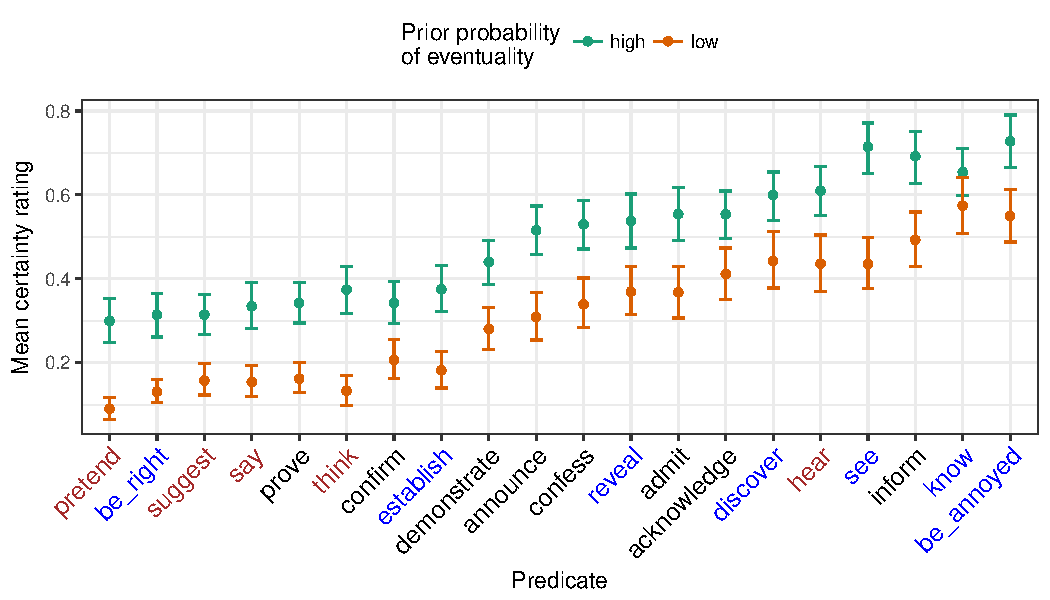
\includegraphics[width=.5\paperwidth]{../results/3-projectivity/graphs/means-projectivity-by-predicate-and-facttype}

\caption{Mean certainty ratings (and 95\% cis) by predicate and prior event probability}
\label{f-projectivity}
\end{figure}

\newpage

\bibliography{../bibliography}

\end{document}
